\section*{Appendix}

\phantomsection % to make sure the clickable link points to the right page
\addcontentsline{toc}{section}{Appendix} % adds this label to the ToC

\subsection{Model documentation}

\subsubsection{Overview}
The French power model FLORE is a dispatch and investment model of the French power mix. It is a partial equilibrium model of the wholesale electricity market, which determines optimal investment and hourly generation.

FLORE minimizes total cost with respect to investment and production under a set of constraints. The model is linear, deterministic, and solved in hourly time step for each year, from 2014 to 2050.

Generation is modelled as twelve distinct technologies: three VRE with zero marginal costs - onshore wind, offshore wind and solar, three fossil-based thermal technologies - coal, combined cycle gas turbine (CCGT), open cycle gas turbine (OCGT), three nuclear technologies (historical nuclear, retrofitted nuclear and new nuclear), and three hydro systems - run-of-river, conventional dams (lakes) and pumped storage. 
Hourly VRE generation is limited by specific generation profiles.
Dispatchable power plants produce whenever the price is above their variable costs, and unless they are limited by their ramping constraints.
Hydro storage and dispatch is optimized by the model, under water reservoir constraints and pumping losses.
At the end its lifetime, each capacity is decommissioned.

A particularity of the model is to represent explicitly the cost of extending the lifetime of nuclear power plants. Nuclear plants normally close after 40 years, but their lifetime can be extended to 60 years, if upgrade costs are paid for.

Demand is exogenous and assumed to be perfectly price inelastic at all times.

FLORE is currently calibrated for France. Exports are given exogenously.

\subsubsection{Total System Costs}

The model minimizes total system costs $C$ with respect to several constraints and decision variables. Total system costs are the sum of fixed costs (representing the sum of capital and fixed O\&M costs), and variable costs, over all hours $h$, weeks $w$, years $y$ and generation technologies $tec$. 

Fixed costs are the product of the capacity installed $CAPA_{tec,y}$ for each technology in year $y$, by its annualized capacity cost $c_{tec}^{inv}$ plus fixed O\&M costs $c_{tec}^{qfix}$. 
Variable generation costs are the product of $GENE_{tec,w,y,h}$, the generation from technology $tec$ in year $y$, week $w$ and hour $h$, by variable generation costs $c_{tec}^{var}$.
\begin{equation}
C =\sum_{tec,y} CAPA_{tec,y} \cdot ( c_{tec}^{inv} + c_{tec}^{qfix} ) + \sum_{tec,y,w,h} GENE_{tec,y,w,h} \cdot c_{tec}^{var}
\end{equation}
Throughout this model description, capital letters denote choice variable for the model, while lowercase letters denote exogenous data.

\subsubsection{Supply and demand}

Power balance between supply and demand is the central constraint of the model. Demand is the sum of national load $d$, pumping for pumped-storage hydro $PUMP$ and exports flow $flows$. 
Supply is the sum of generation over all technologies.
$$\forall h,y \quad \sum_{tec} GENE(tec,h,y) \geq \sum_{tec} LOAD(h,y) + PUMP(h,y) + flow(h,y)$$

In this framework, demand is perfectly price-inelastic. Cost minimization is thus equivalent to welfare-maximization.

Generation is constrained by capacities installed and the load factor (also called availability), for all technologies except wind, PV and run-of-river hydro, which present a specific generation profile.
$$GENE(tec\_noprof,y,w,h) \leq CAPA(tec\_noprof,y)*loadfactor(tec\_noprof)$$
For wind and PV, a generation profile is an additional constraint:
$$GENE(tec\_res,y,w,h) \leq CAPA(tec\_res,y)*res\_profiles(h,tec\_res)$$
For run-of-river hydro, generation is fixed exogenously for each week:
$$GENE("river",y,w,h) = river\_flow(w)$$

Investment is exogenous for historical nuclear and the three hydro technologies. The capacity of historical nuclear technology is decreasing based on plant-level data, with each plant capacity being phased-out when it reaches 40 years old. For hydro, we assume constant capacities for run-of-river and lakes. Pumped-hydro potential is expected to grow by 3.2GW by 2050, starting from 5 GW in 2014, with a discharge time of 20 hours, as in ADEME (Visions ADEME 2030).
$$CAPA_{tec\_ex,y} = capa_exo_{y,tec\_ex} $$

The capacity of all other technologies is determined endogenously by the model. Capacity is installed when optimal, and then decommissioned when it reaches its lifetime. The initial capacity, already installed in 2014, is supposed to be decommissioned linearly from 2014 onwards in a period of 40 years.
\begin{align*}
CAPA_{tec\_end,y+1} &= CAPA_{tec\_end,y} + INVE_{tec\_end,y} - DECO\_{tec\_end,y} \\
DECO_{tec\_end,y}  &= INVE_{tec\_end,y-lifetime(tec\_end)} + (tec\_data_{tec\_end,'initcap'}/40)\$(ord(y) <= 40) 
\end{align*}



\subsubsection{Power System Inflexibilities}

The model includes ramp-up and ramp-down constraints for nuclear and coal power plants, to represent the fact that generation cannot vary too quickly from one hour to the next. These constraints are modelled as a maximum variation rate:
The ramp up constraint is:
$$\forall tec\_ramp,y,w,h \quad GENE(tec\_ramp,y,w,h+1) \leq GENE(tec\_ramp;y;w;h) \dot (1+ramp\_rate)$$
The ramp-down constraint is:
$$\forall tec\_ramp,y,w,h \quad GENE(tec\_ramp,y,w,h+1) \geq GENE(tec\_ramp;y;w;h) \dot (1-ramp\_rate)$$
We take the value of $0.08$ for coal and $0.05$ for nuclear - for both ramp-up and ramp-down, as in \citet{ADEME2015}.

\subsubsection{Model limitation}

This model was design to model the French power system from 2014 to 2050, optimizing investment and dispatch over many assumptions on nuclear costs. As such, it had to make several simplifying assumptions.

This model does not provide a detailed representation of infra-hourly events. In particular, ancillary services are not represented. 

We do not model power plants at the plant level, but we rather use representative technologies. Thus, one limitation is the absence of constraints related to unit commitment, such as start-up cost and delay, minimum load, and part-load efficiency. 
However, this default is in part compensated for nuclear. We use real data on age limit (or retirement), so the model retrofits plants whose capacity is in line with plant-level data. On the contrary, new nuclear will be installed continuously, while in reality it composed of discrete power plants with a significant size (1.3 GW for the EPR technology).
For renewable, the representative technology assumption is less of an issue as these technologies are modular, and very small in size. The continuous approach is here a good assumption for costs. However, this approach does not enable one to distinguish the different potentials within a country, both for solar and wind. 

%%%%%%%%%%%%%%%%

\clearpage

\subsubsection{Model Calibration}

\label{app:calibration}

The model is calibrated using capital cost, fixed O\&M and variable O\&M costs. All payments are annualized with a 5\% interest rate. The corresponding LCOE with usual load factor are given in the Figure \ref{fig:calibration_LCOE}.

\begin{figure}[!ht]
	\centering
	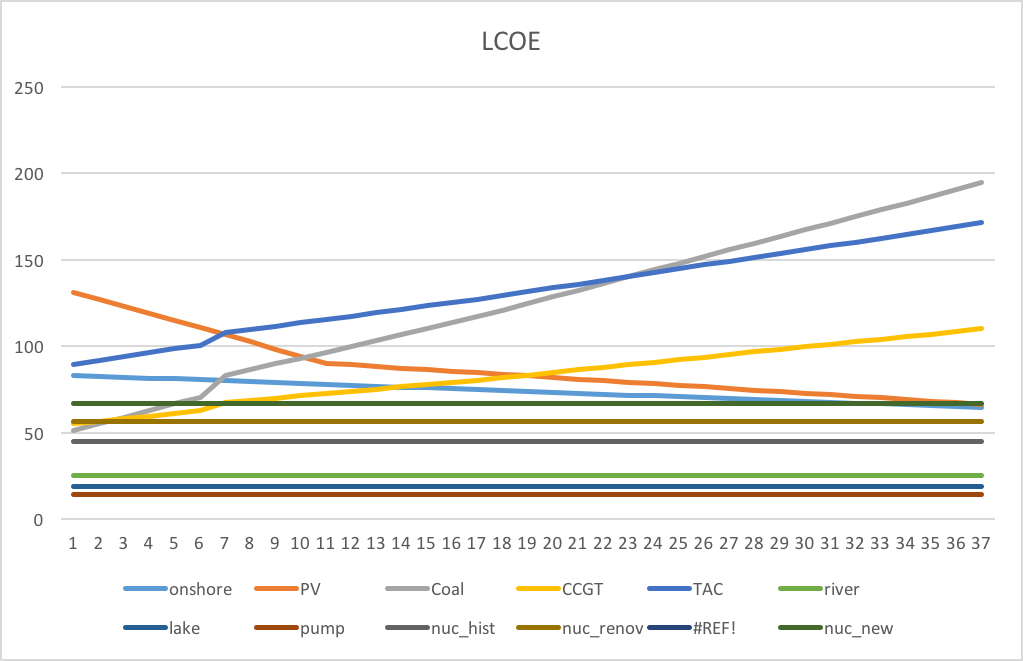
\includegraphics[width=12cm]{figures/calibration_LCOE.png}
	\caption{LCOE computed from input data of the model}
	\label{fig:calibration_LCOE}
\end{figure}

\begin{table}[!ht]
	%\colorTable
	\centering
	\caption{Main model parameters}
	\begin{tabular}{llr}
		\toprule
		parameter&value&unit\\
		\midrule
		Rate of pure time preference &0&\%\\
		Financial interest rate&5&\%\\
		\bottomrule
	\end{tabular}
\end{table}

\begin{table}[!ht]
	\centering
	\caption{Investment costs (euros/kW)}
	\label{tab:Investment _costs}
	\begin{adjustbox}{width=1\textwidth}
	\small
	\begin{tabular}{llllllllllll}
		\toprule
		 Year & onshore & PV & Coal & CCGT & TAC & river & lake & pump & nuc\_hist & nuc\_renov & nuc\_new \\
		\midrule
		2014 & 1650 & 1560 & 1500 & 800 & 400 & 3000 & 2000 & 2000 & 1320 & 1938 & 6000 \\
		2020 & 1572 & 1194 & 1500 & 800 & 400 & 3000 & 2000 & 2000 & 1320 & 1938 & 6000 \\
		2030 & 1443 & 869 & 1500 & 800 & 400 & 3000 & 2000 & 2000 & 1320 & 1938 & 6000 \\
		2040 & 1313 & 735 & 1500 & 800 & 400 & 3000 & 2000 & 2000 & 1320 & 1938 & 6000 \\
		2050 & 1184 & 600 & 1500 & 800 & 400 & 3000 & 2000 & 2000 & 1320 & 1938 & 6000 \\
		\bottomrule
	\end{tabular}
\end{adjustbox}
\end{table}

\begin{table}[!ht]
	\centering
	\caption{Fixed O\&M costs (euro/MWh)}
	\label{tab:OM_costs}
		\begin{adjustbox}{width=1\textwidth}
	\small
	\begin{tabular}{llllllllllll}
		\toprule
		Year & onshore & PV & Coal & CCGT & TAC & river & lake & pump & nuc\_hist & nuc\_renov & nuc\_new \\
		\midrule
		2014 & 35 & 25 & 30 & 20 & 15 & 60 & 60 & 20 & 188 & 188 & 100 \\
		2020 & 35 & 25 & 30 & 20 & 15 & 60 & 60 & 20 & 188 & 188 & 100 \\
		2030 & 35 & 25 & 30 & 20 & 15 & 60 & 60 & 20 & 188 & 188 & 100 \\
		2040 & 35 & 25 & 30 & 20 & 15 & 60 & 60 & 20 & 188 & 188 & 100 \\
		2050 & 35 & 25 & 30 & 20 & 15 & 60 & 60 & 20 & 188 & 188 & 100 \\
		\bottomrule
	\end{tabular}
\end{adjustbox}
\end{table}


\begin{table}
	\centering
	\caption{\coo\ price}
	\label{tab:CO2_price}
	\begin{tabular}{llll}
		\toprule
		Year & \coo\ price & & \\
		\midrule
		& Central & Low & High \\
		2014 & 21 & 10 & 42 \\
		2020 & 28 & 14 & 56 \\
		2030 & 50 & 25 & 100 \\
		2040 & 75 & 38 & 150 \\
		2050 & 100 & 50 & 200 \\
		\bottomrule
	\end{tabular}
\end{table}



\begin{table}[!ht]
	\centering
	\caption{Fuel prices}
	\label{tab:Fuel_prices}
	\begin{tabular}{llll}
		\toprule
		euro/MWh & Coal & Gas & Uranium \\
		\midrule
		2014 & 10,3 & 25,3 & 7,30 \\
		\bottomrule
	\end{tabular}
\end{table}

\begin{table}
	\centering
	\caption{Efficiencies}
	\label{tab:Efficiencies}
	\begin{tabular}{lll}
		\toprule
		Coal & CCGT & TAC \\
		\midrule
		0,43 & 0,61 & 0,410 \\
		\bottomrule
	\end{tabular}
\end{table}

%%%%%%%%%%%%%%%%%%
\clearpage
\subsection{Additional material}

\subsubsection{Plausible costs of retrofitted plants}


\begin{table}
	\centering
	\caption{Historical values of French nuclear plants in the literature, in the best case}
	\label{tab:historical_costs}
	\begin{tabular}{llll}
		\toprule
		Item & Cost & Unit & Source \\
		\midrule
		Historical OPEX & 13.3 & euro/MWh & Boccard, 2014 \\
		Fuel & 5.7 & euro/MWh & Cour des Comptes, 2014, p. 13 \\
		Waste & 3.6 &  & Cour des Comptes, 2014, p. 24 \\
		Decommissioning & 1 &  & Cour des Comptes, 2014, p. 24 \\
		Capital rate & 5 & \% &  \\
		Lifetime extension & 20 & years & \\
		availability & 83.5 & \% & \\
		\bottomrule
	\end{tabular}
\end{table}


\begin{table}
	\centering
	\caption{Retrofit costs according to EDF}
	\label{tab:costs_grand_carenage}
	\begin{tabular}{lll}
		\toprule
		Additional CAPEX & 74730 & million euros \\
		\midrule
		Additional OPEX & 25160 & million euros \\
		Capacity concerned & 53200 & MW \\
		\bottomrule
	\end{tabular}
\end{table}


\begin{table}
	\centering
	\caption{Sensitivity tests}
	\label{tab:sensitivity_tests}
	\begin{tabular}{lll}
		\toprule
		CAPEX & 30 & \% \\
		\midrule
		Historical OPEX & 27.5 & euro/MWh \\
		Capital rate & 10 & \% \\
		Lifetime extension & 10 & years \\
		Availability & 70 & \% \\
		Waste & x2 &  \\
		Decommissioning & x2 &  \\
		Insurance & 8.5 & euro/MWh \\
		\bottomrule
	\end{tabular}
\end{table}



\subsubsection{Strategies examined}
\label{sec:strategies_examined}

\begin{figure}[!ht]
	\centering
	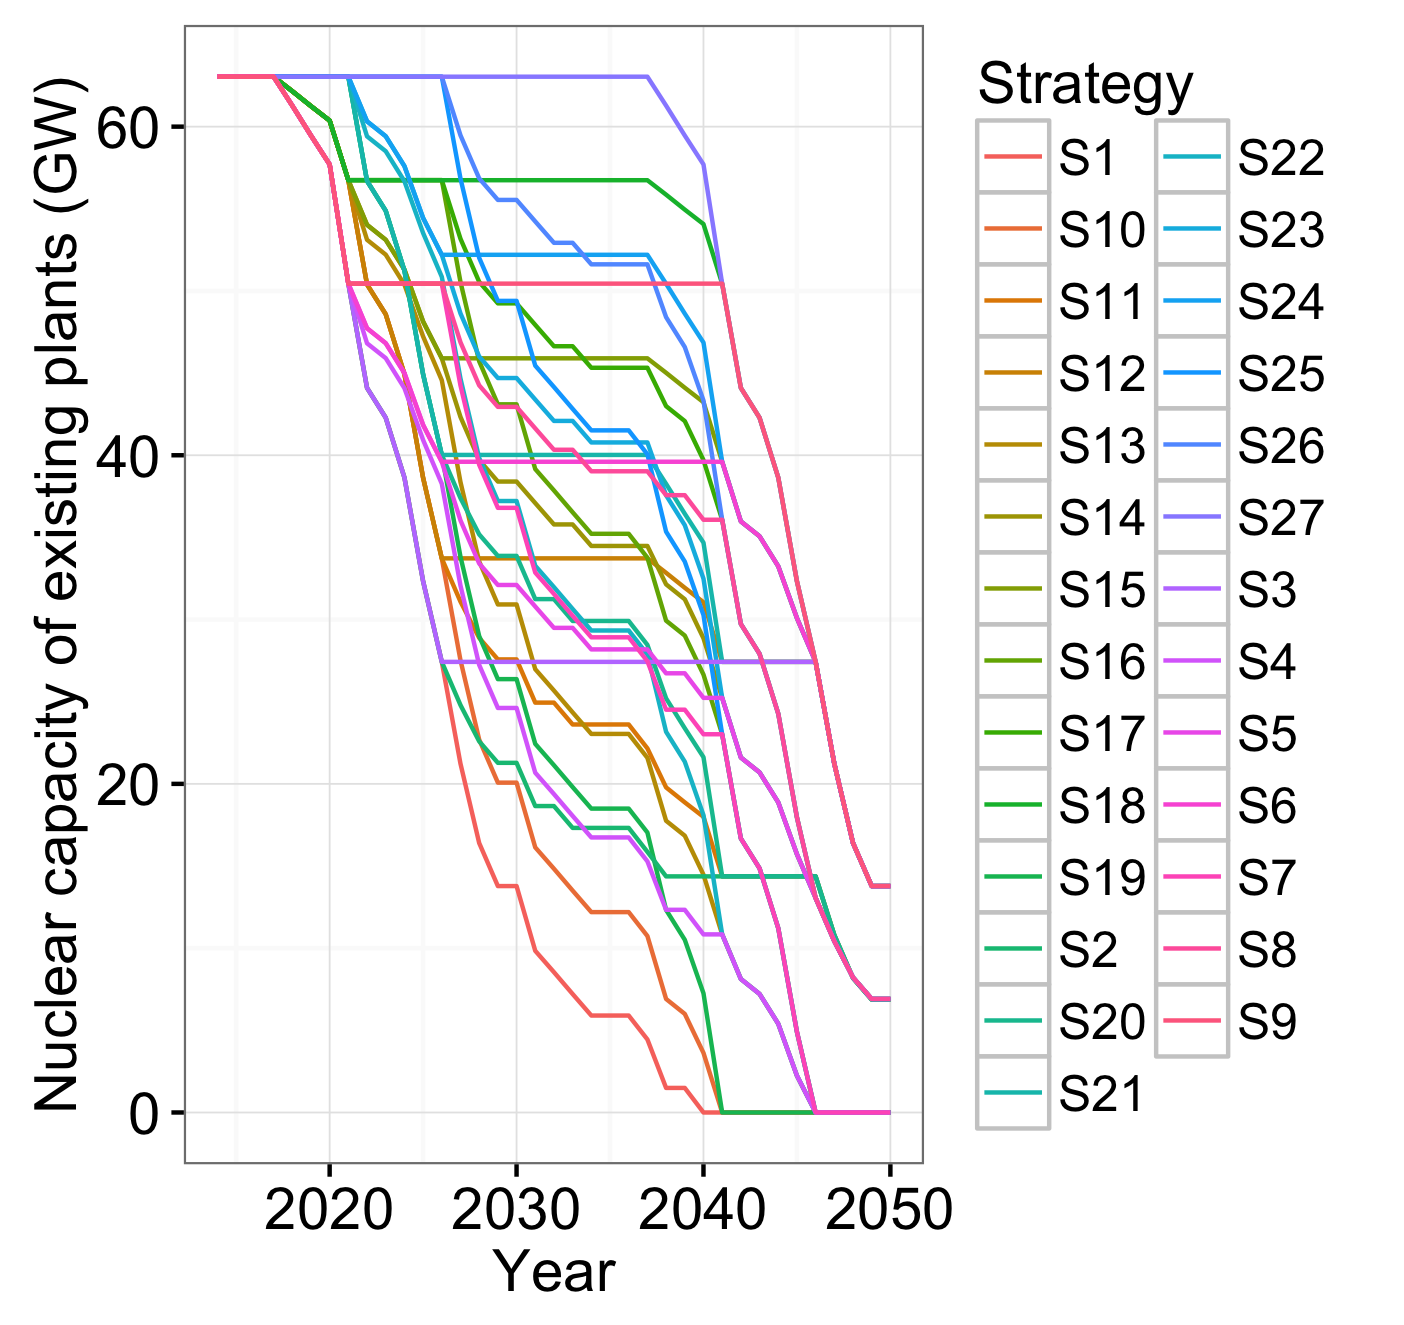
\includegraphics[height=7cm]{figures/strategies.png}
	\caption{Nuclear capacity of existing plants, including retrofit, in the 27 strategies}
	\label{fig:strategies}
\end{figure}

\clearpage

\begin{table}
	\centering
	\caption{Share of retrofitted nuclear plants in each period}
	\label{tab:shareNukeRetrofit}
	\begin{tabular}{llll}
		\toprule
		Strategy & Period1 & Period2 & Period3 \\
		\midrule
		S1 & 0\% & 0\% & 0\% \\
		S2 & 0\% & 0\% & 50\% \\
		S3 & 0\% & 0\% & 100\% \\
		S4 & 0\% & 50\% & 0\% \\
		S5 & 0\% & 50\% & 50\% \\
		S6 & 0\% & 50\% & 100\% \\
		S7 & 0\% & 100\% & 0\% \\
		S8 & 0\% & 100\% & 50\% \\
		S9 & 0\% & 100\% & 100\% \\
		S10 & 50\% & 0\% & 0\% \\
		S11 & 50\% & 0\% & 50\% \\
		S12 & 50\% & 0\% & 100\% \\
		S13 & 50\% & 50\% & 0\% \\
		S14 & 50\% & 50\% & 50\% \\
		S15 & 50\% & 50\% & 100\% \\
		S16 & 50\% & 100\% & 0\% \\
		S17 & 50\% & 100\% & 50\% \\
		S18 & 50\% & 100\% & 100\% \\
		S19 & 100\% & 0\% & 0\% \\
		S20 & 100\% & 0\% & 50\% \\
		S21 & 100\% & 0\% & 100\% \\
		S22 & 100\% & 50\% & 0\% \\
		S23 & 100\% & 50\% & 50\% \\
		S24 & 100\% & 50\% & 100\% \\
		S25 & 100\% & 100\% & 0\% \\
		S26 & 100\% & 100\% & 50\% \\
		S27 & 100\% & 100\% & 100\% \\
		\bottomrule
	\end{tabular}
\end{table}

The first period includes all reactors that reach 40 years before 2021, which represents 14 reactors. The second period includes all the reactors reaching 40 years between 2021 and 2025, which represent 23 addditional reactors. The final period goes up to 2050 and represents the remaining 21 reactors.
\subsubsection{Optimum power mixes}
\label{app:optimumMixes}


\begin{figure}
	\centering
	\subfloat[Optimum for retrofitted nuclear below or equal to 40 \emwh] {
		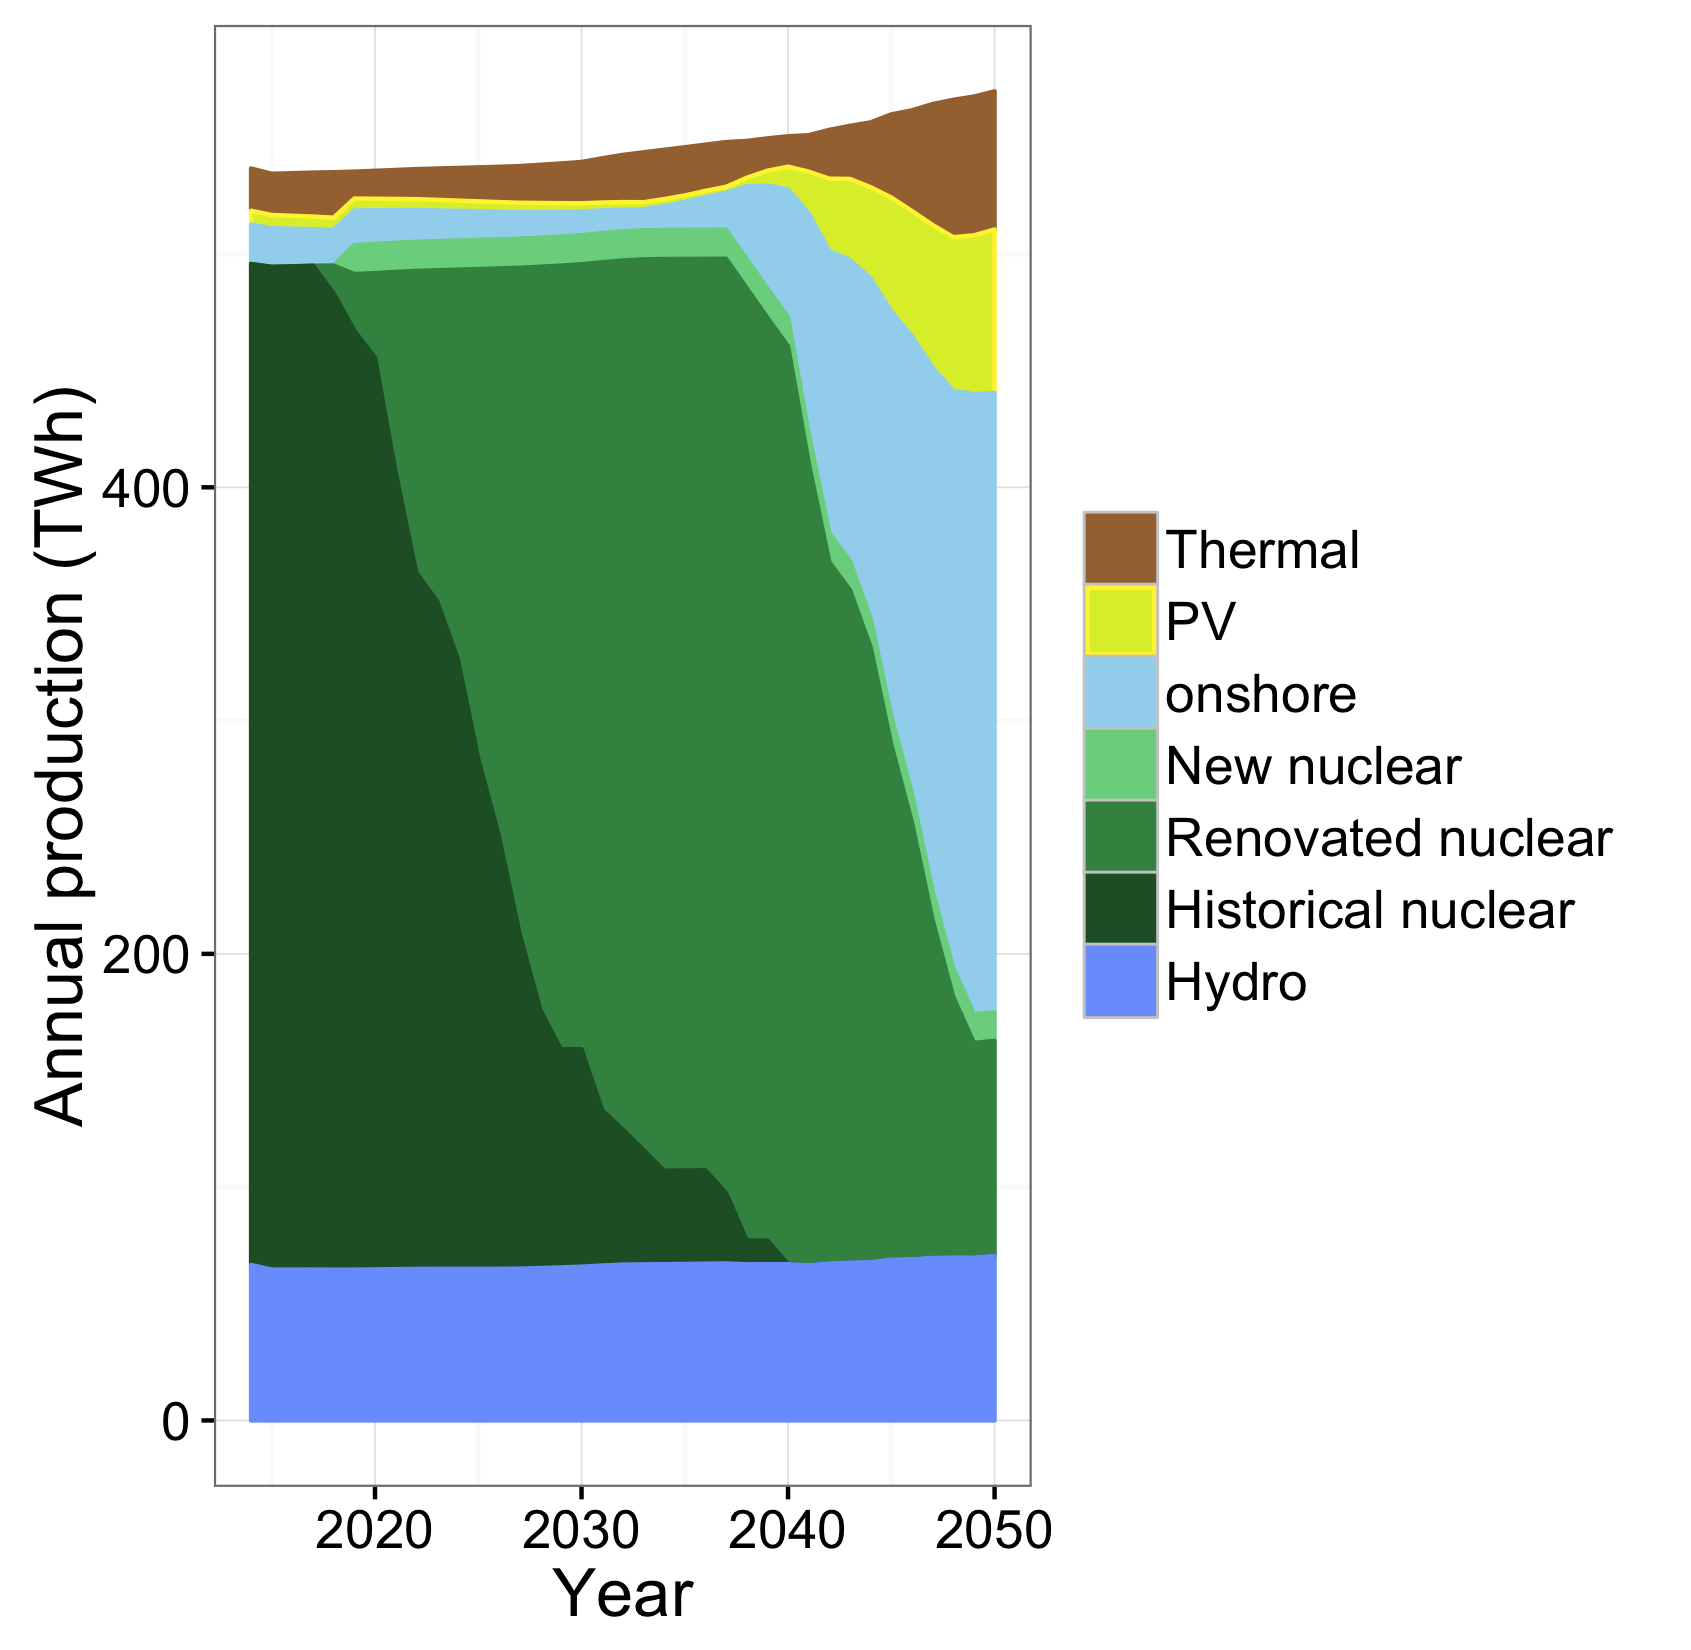
\includegraphics[width=7cm]{figures/powerMix_R40N100MedD.png}
		\label{fig:nukeShare40}
	}
	\subfloat[Optimum for retrofitted nuclear around 70 \emwh] {
		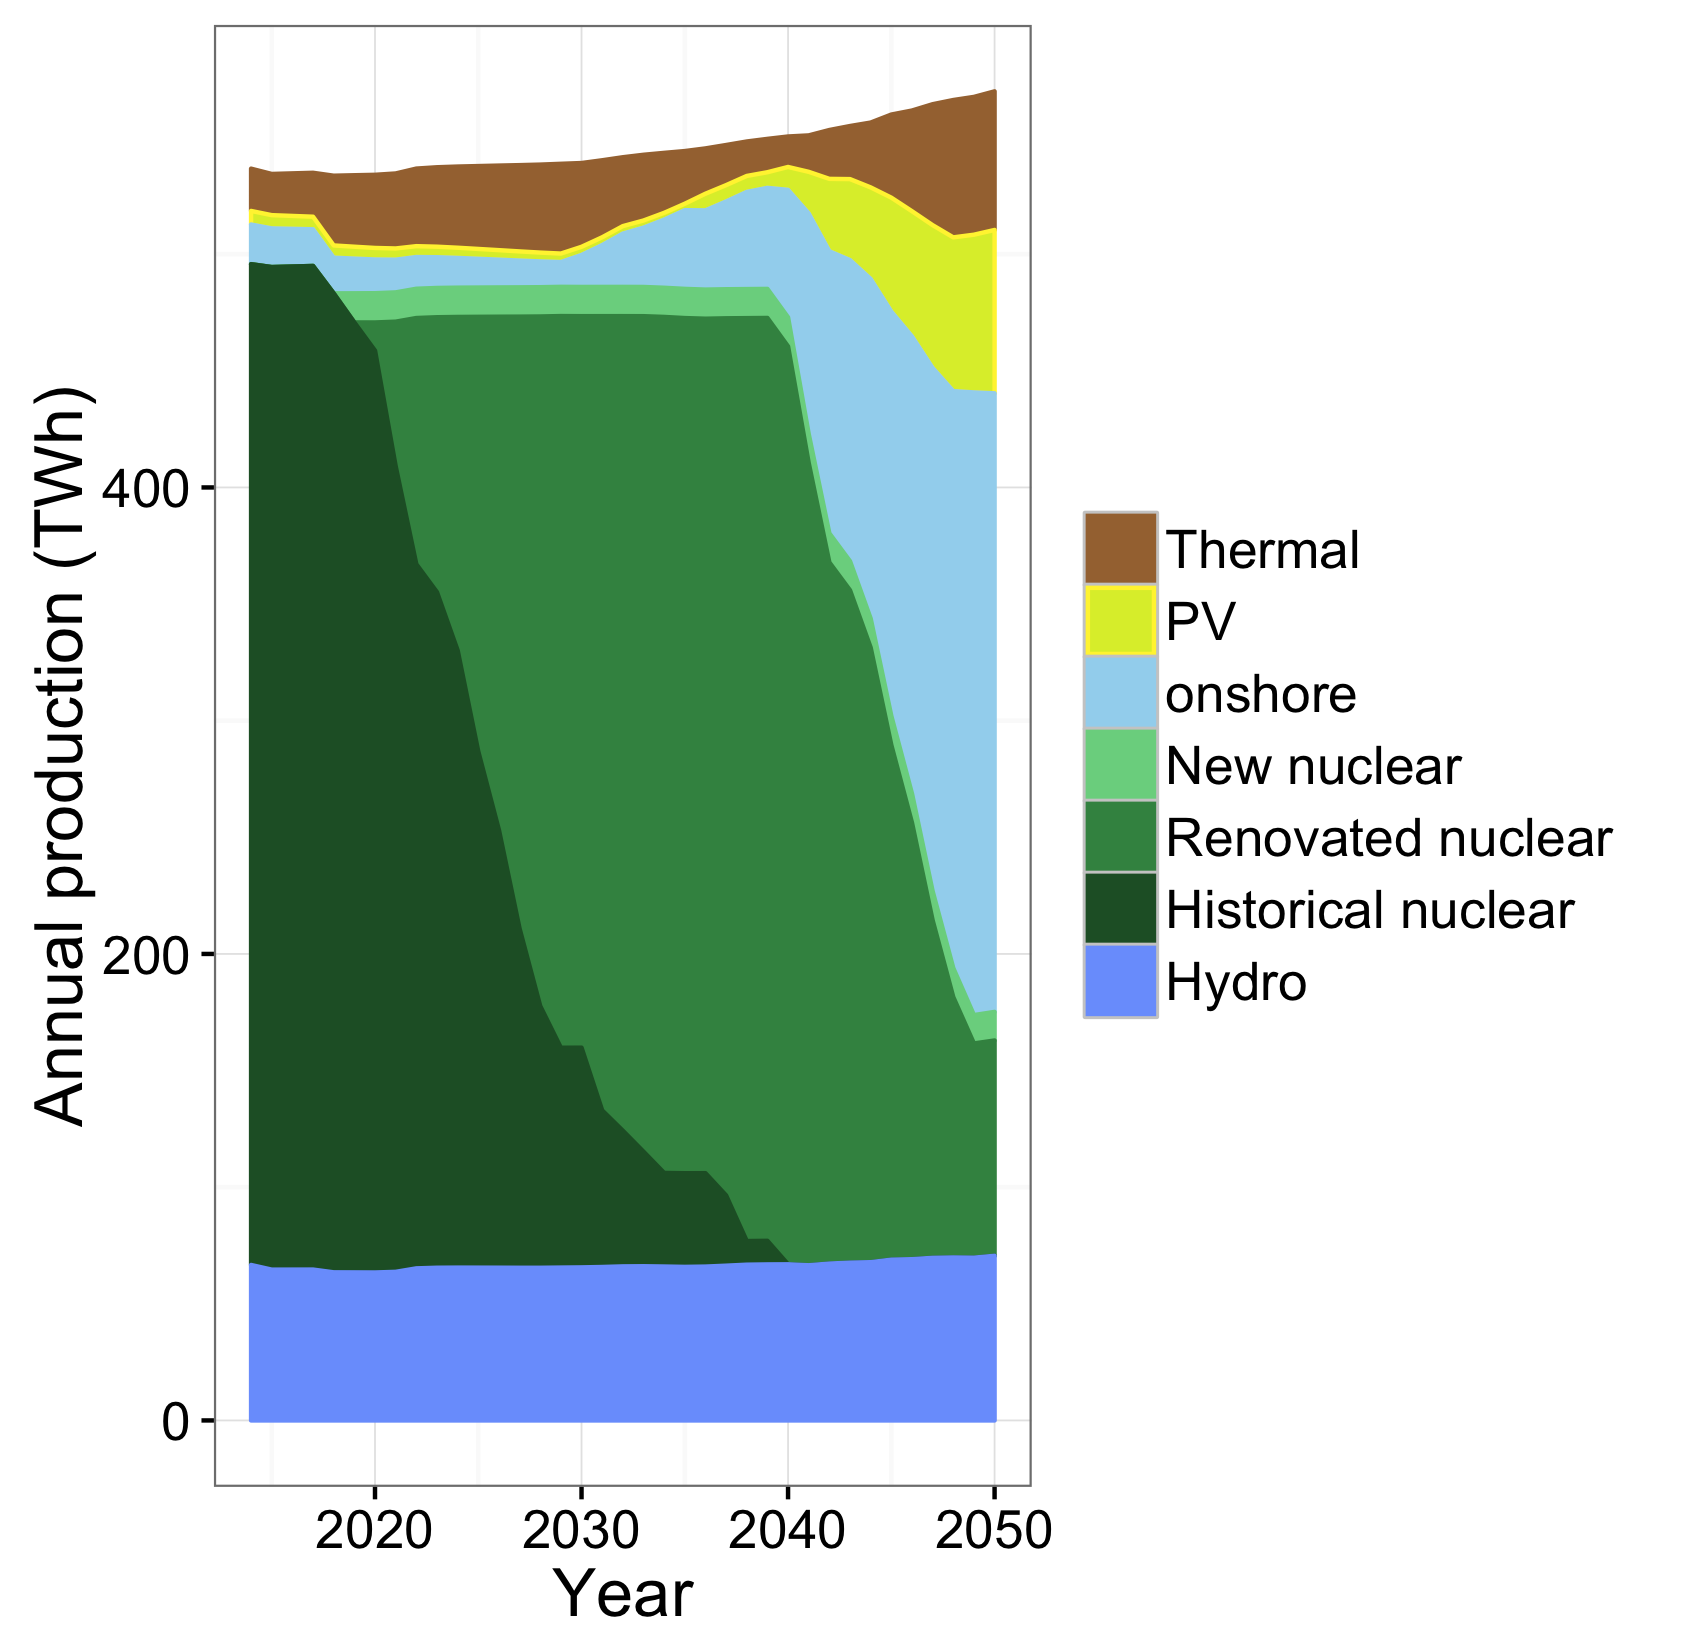
\includegraphics[width=7cm]{figures/powerMix_R70N100MedD.png}
		\label{fig:nukeShare70}
	}
\end{figure}

\begin{figure}
	\centering
		\subfloat[Optimum for retrofitted nuclear around 80 \emwh] {
		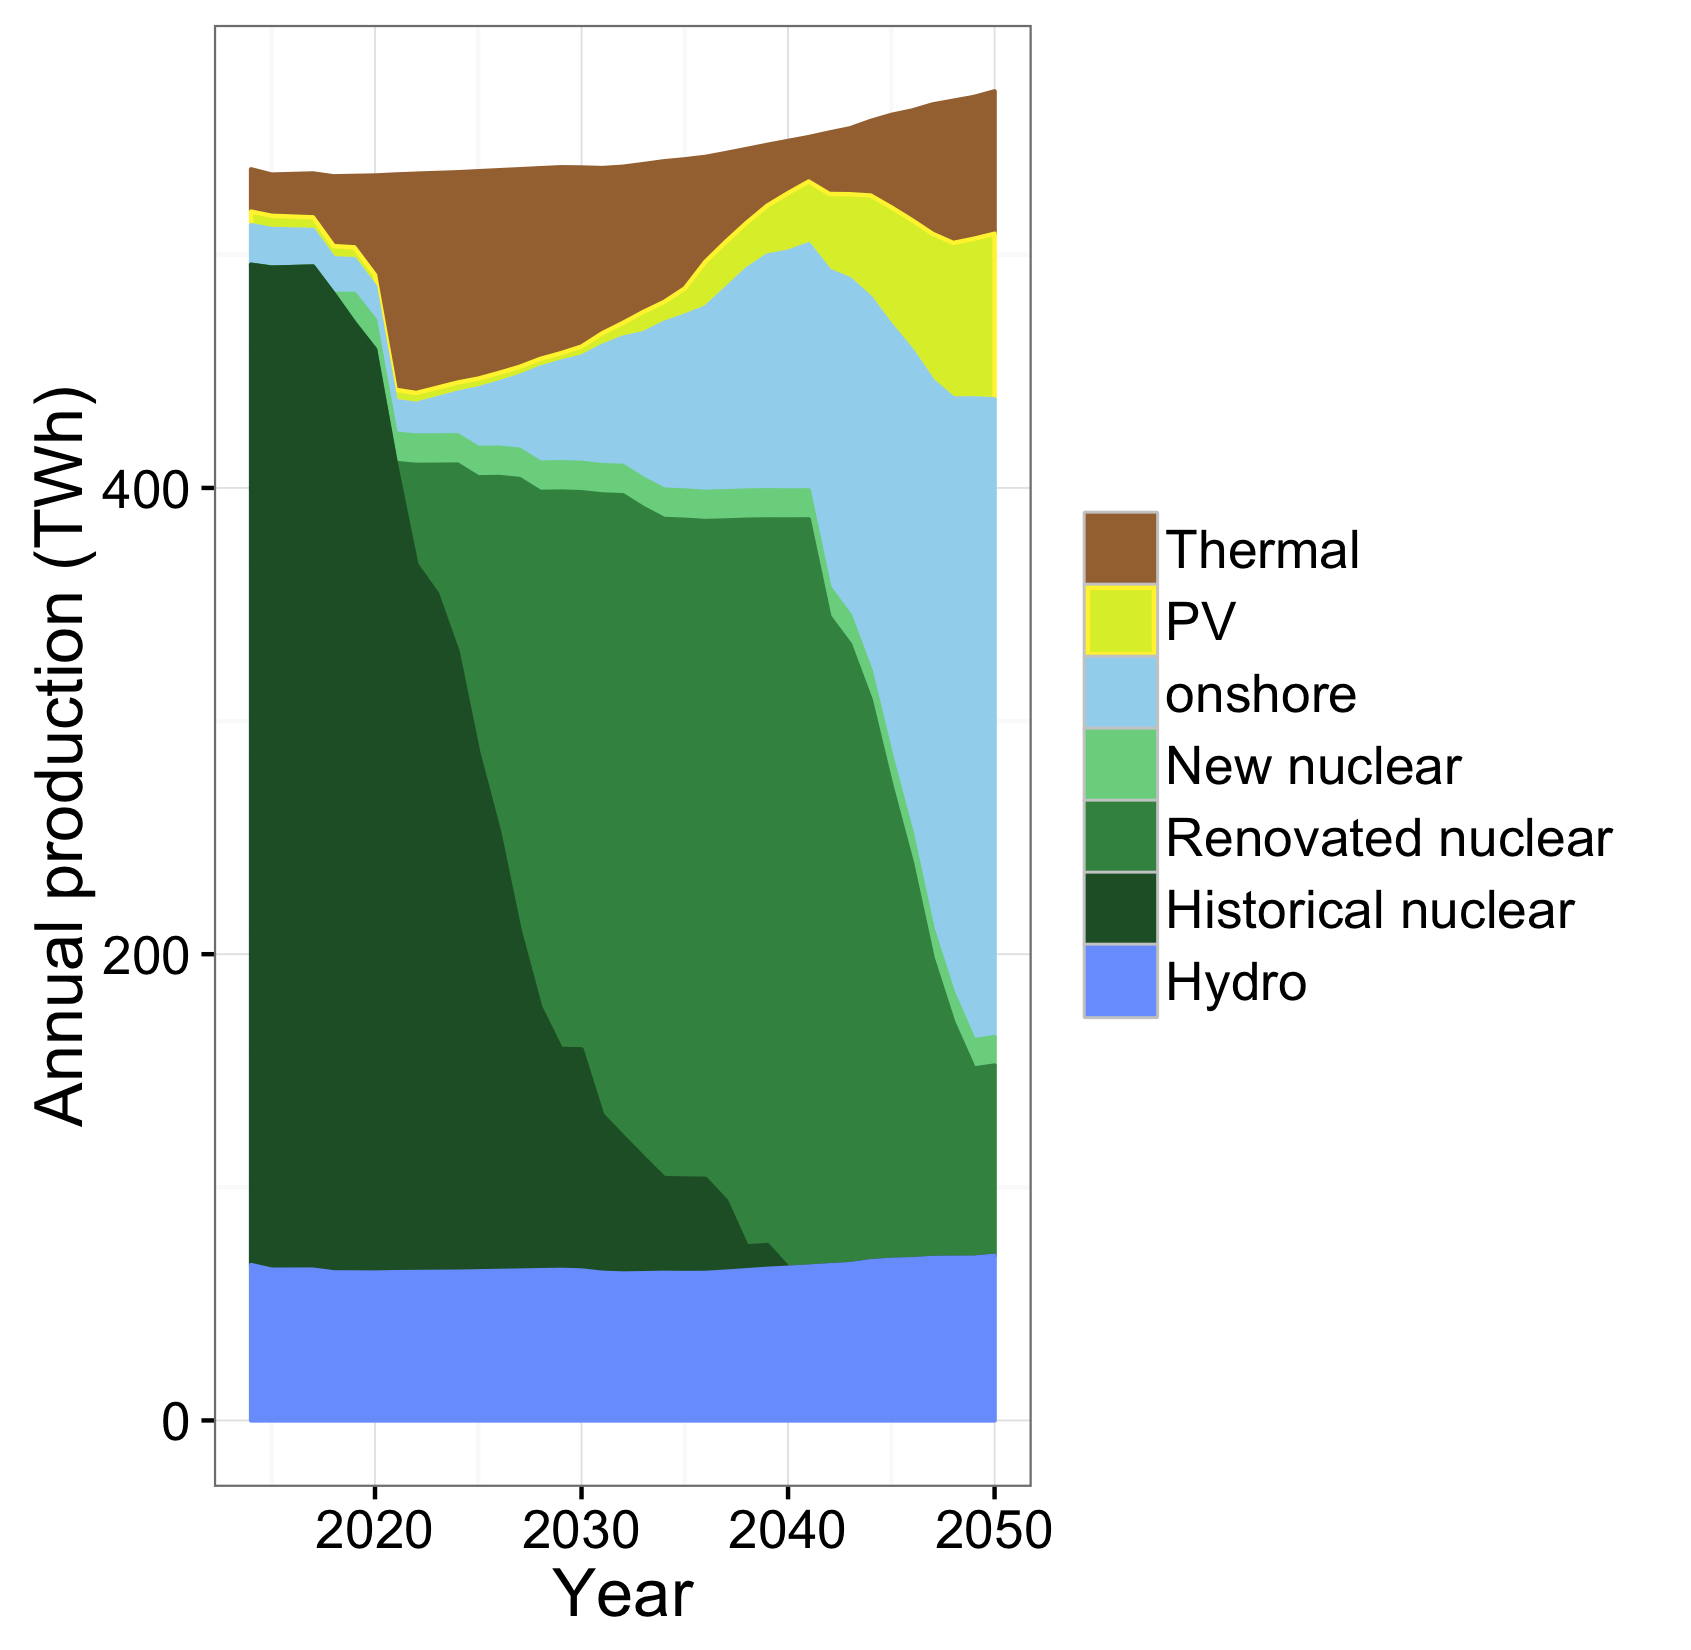
\includegraphics[height=8cm]{figures/powerMix_R80N100MedD.png}
		\label{fig:nukeShare80}
	}
	\subfloat[Optimum for retrofitted nuclear around 90 \emwh] {
		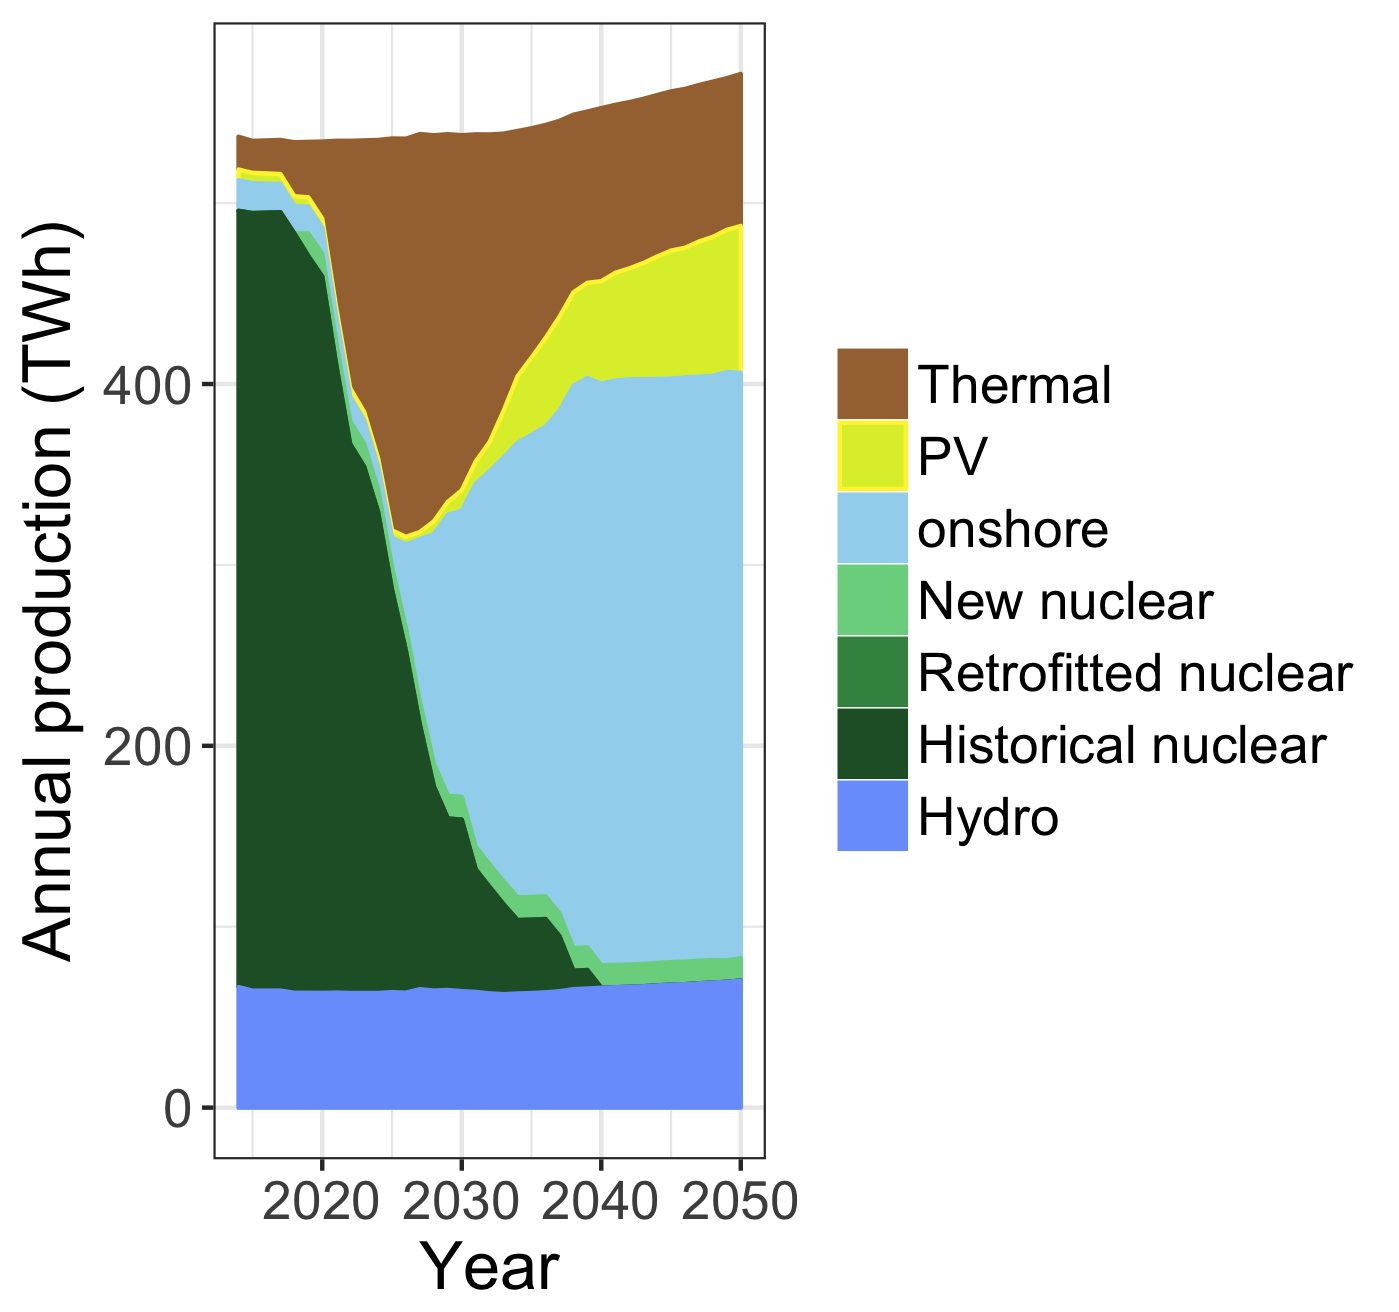
\includegraphics[height=8cm]{figures/powerMix_R90N100MedD.png}
		\label{fig:nukeShare90}
	}
	\caption{Optimum power mix for various nuclear retrofitting costs}
\end{figure}


\begin{figure}[!ht]
	\centering
	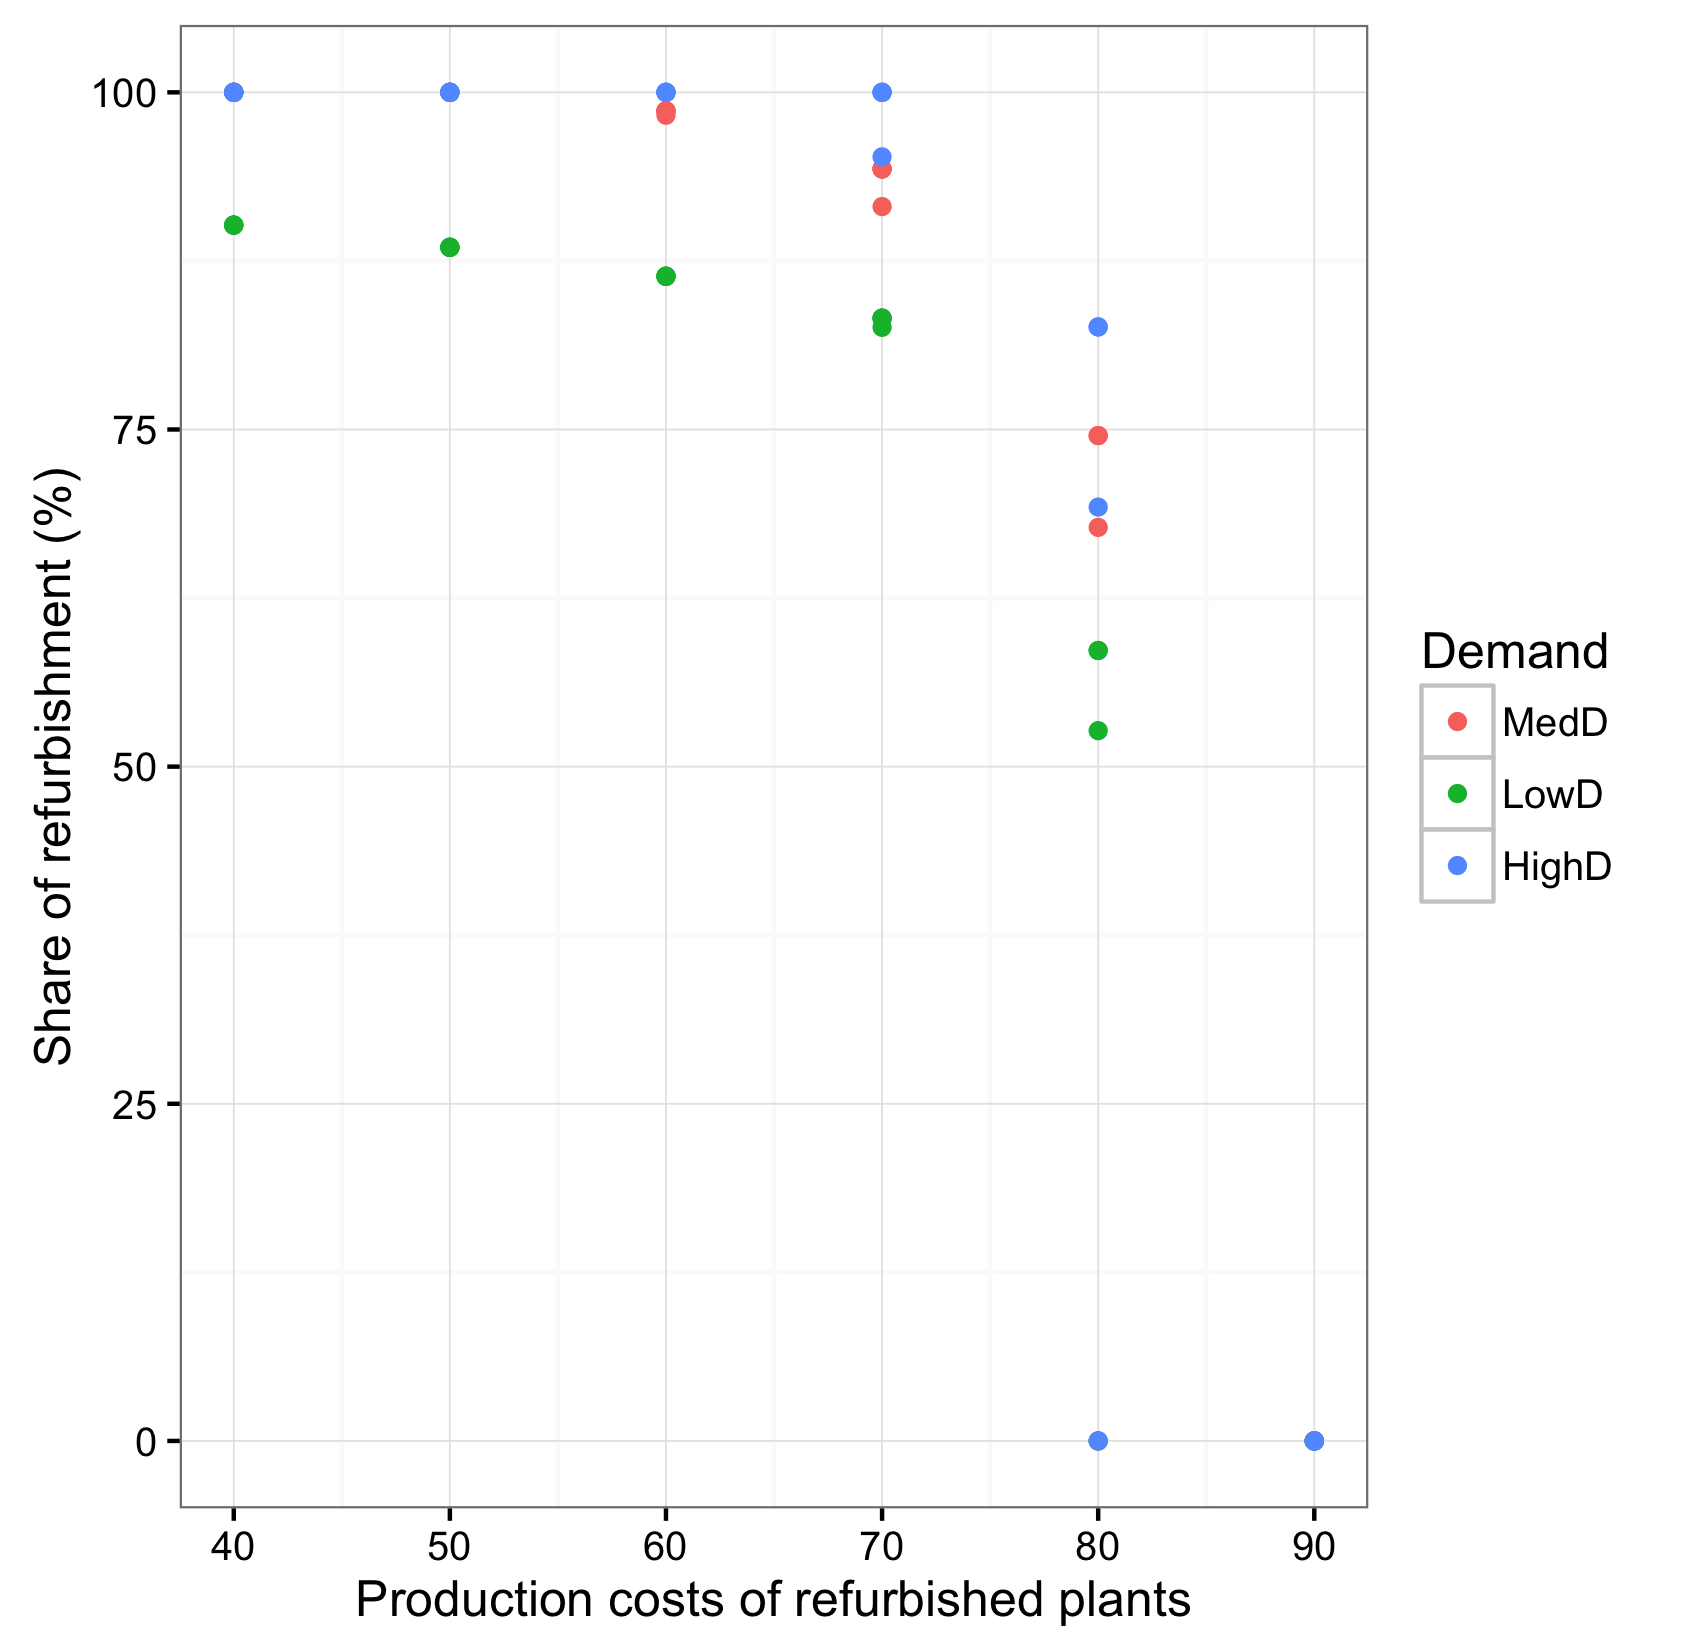
\includegraphics[height=8cm]{figures/powerMixSensitivity.png}
	\caption{Optimal nuclear shares and sensitivity analysis}
	\label{fig:powerMixSensitivity}
\end{figure}


%%%%%%%%%%%%

\clearpage

\subsubsection{Analysis with PRIM}


\subsubsection{Choice of threshold}

\begin{figure}
	\centering
	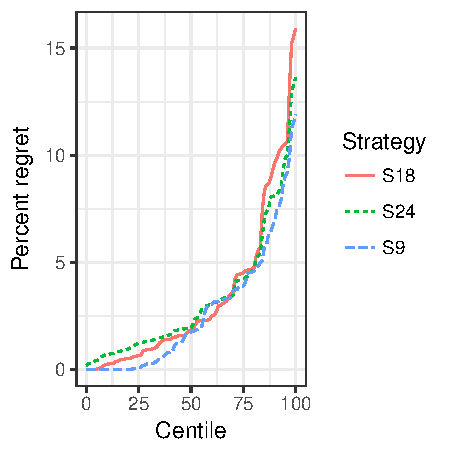
\includegraphics[width=6cm]{figures/quantile_regret.pdf}
	\caption{Ordered distribution of regret for the three candidate strategies S9, S24 and S18}
	\label{fig:quantile_regret}
\end{figure}



\subsubsection{Efficiency frontier}

\begin{figure}
	\centering
	\subfloat[With the cluster from S9] {
		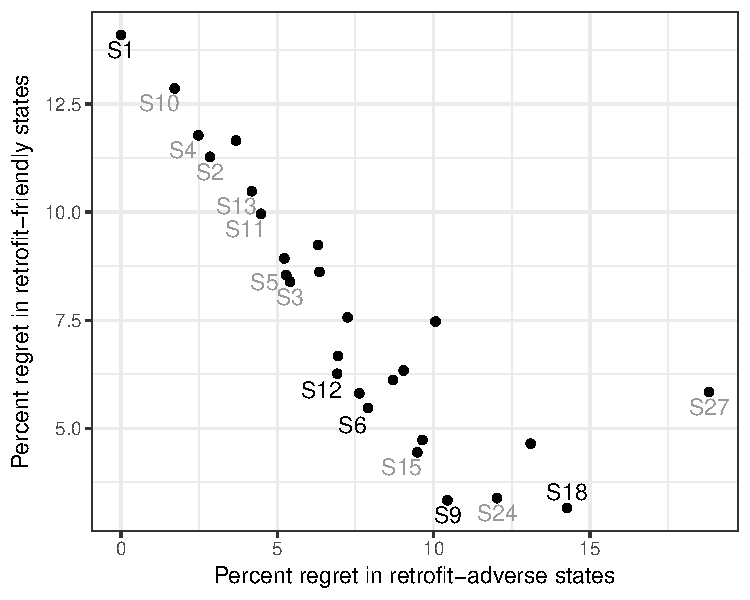
\includegraphics[width=6cm]{figures/low_regret_frontier_S9.pdf}
	}
\subfloat[With the cluster from S18 and S24] {
		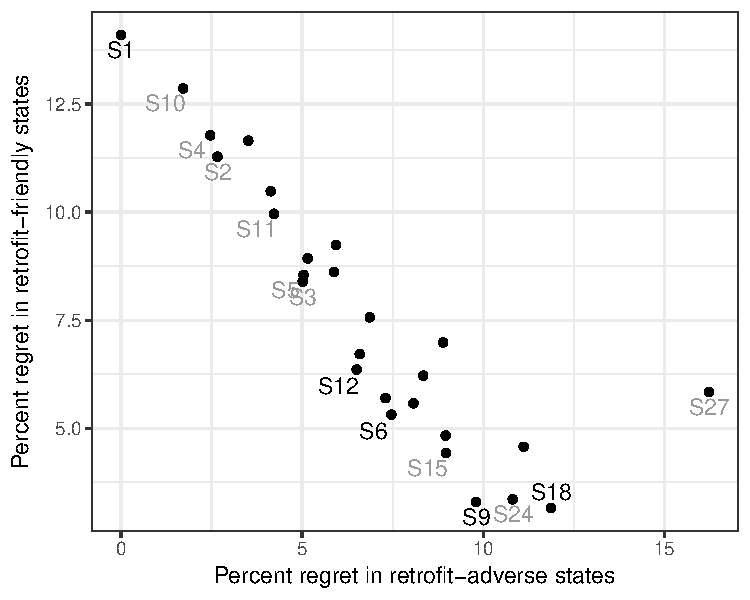
\includegraphics[width=6cm]{figures/low_regret_frontier_S18.pdf}
}
	\caption{Trade-offs and efficiency fontier using the PRIM-generated cluster from strategy S9 and strategy S18 and S24}
	\label{fig_app:low_regret_frontier}
\end{figure}


\subsubsection{Regrets of the strategies S9, S18 and S27}


\begin{figure}
	\centering
	\subfloat[Regret of the full-retrofit strategy S27] {
		\makebox[5.5cm][c]{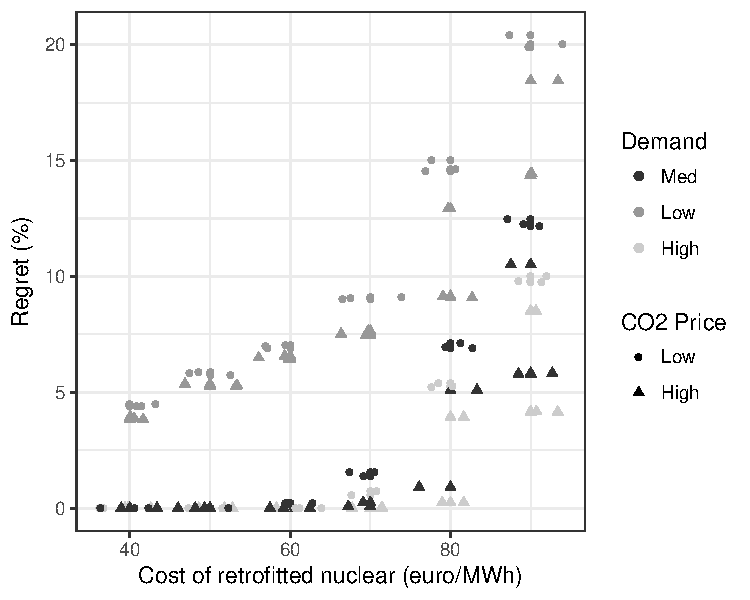
\includegraphics[height=5cm]{figures/vulnerabilities_S27.pdf}}
		\label{fig_app:vulnerabilities_S27}
	} 

	\subfloat[Regret of the full-retrofit strategy S9] {
		\makebox[5.5cm][c]{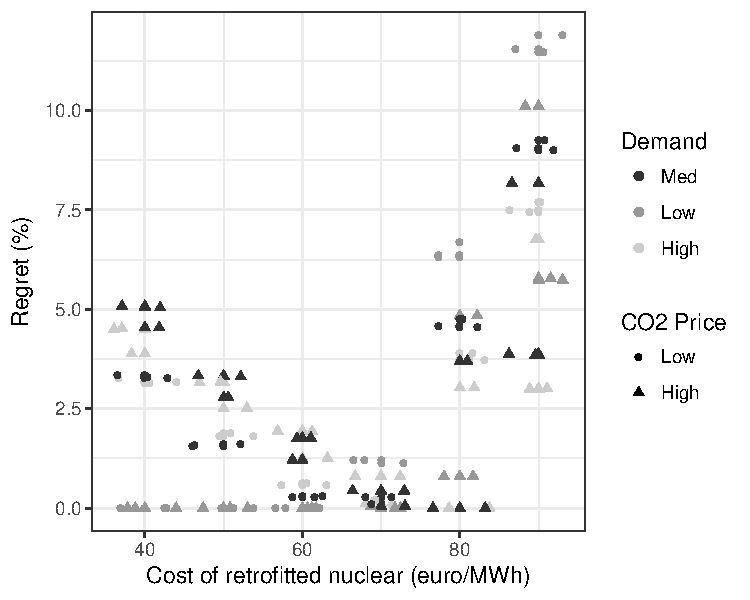
\includegraphics[height=5cm]{figures/vulnerabilities_S9.pdf}}
	} \qquad
	\subfloat[Regret of the full-retrofit strategy S18]{
		\makebox[6cm][c]{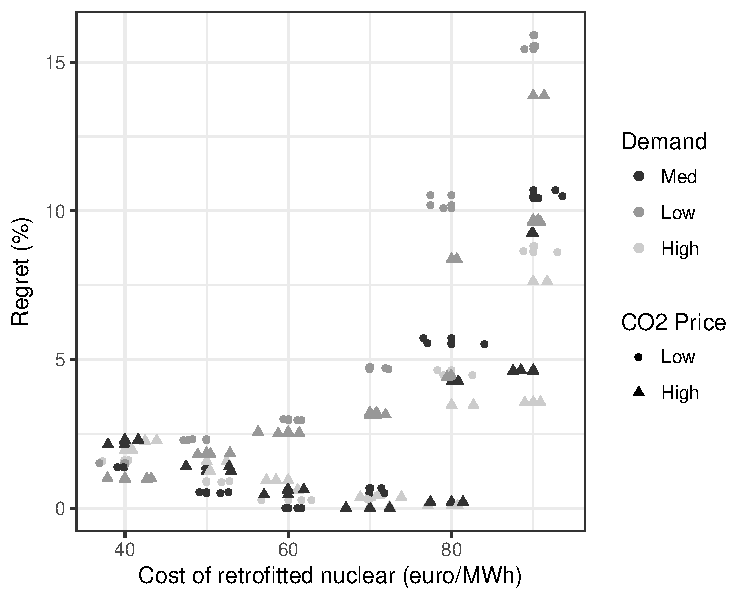
\includegraphics[height=5cm]{figures/vulnerabilities_S18.pdf}}
		\label{fig_app:vulnerabilities_S9_S18_S27}
	}
	\caption{Regret of the full-retrofit strategy S9, S18 and S27}
\end{figure}

\subsubsection{Optimal trajectory depending on implicit probabilities}

\begin{figure}
	\centering
	\subfloat[With the cluster from strategy S9] {
		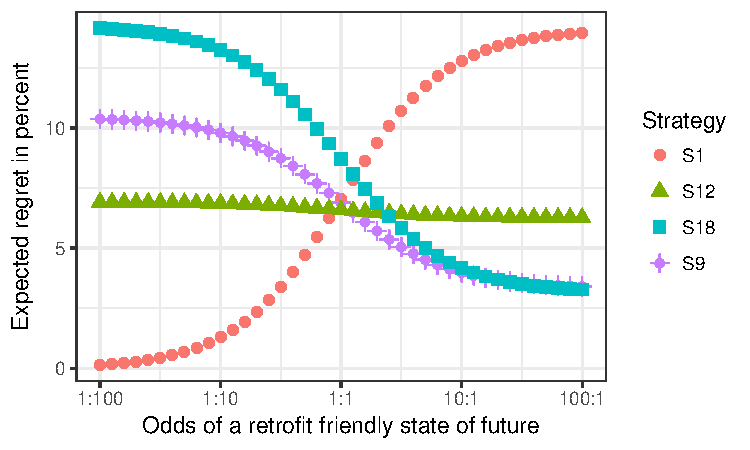
\includegraphics[width=6cm]{figures/odds_S9.pdf}	
	}
	\subfloat[With the cluster from strategy S18 and S24] {
		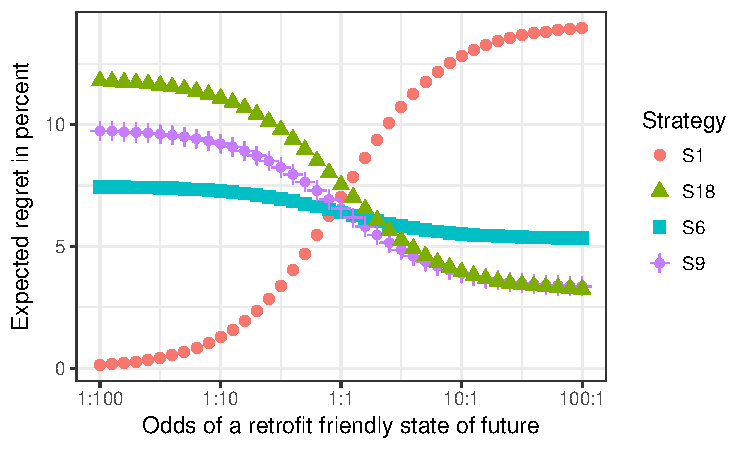
\includegraphics[width=6cm]{figures/odds_S18.pdf}	
	}
	\caption{Optimal strategy depending on the implicit odds of the decision maker}
	\label{fig_app:odds}
\end{figure}


%%%%%%%%%%%%%%%%%%%%%%%%%%%%ù
\clearpage
\subsubsection{Comparison with official scenarios}

\begin{figure}
	\centering
	\subfloat[Nuclear share (\%)] {
		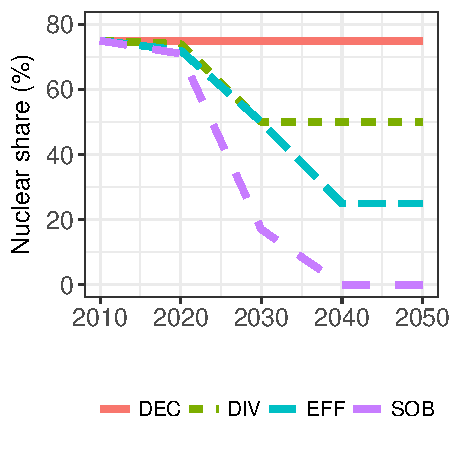
\includegraphics[height=6cm]{figures/dnte_nuc_shares.pdf}
	}
\subfloat[Demand levels (TWh/year)] {
		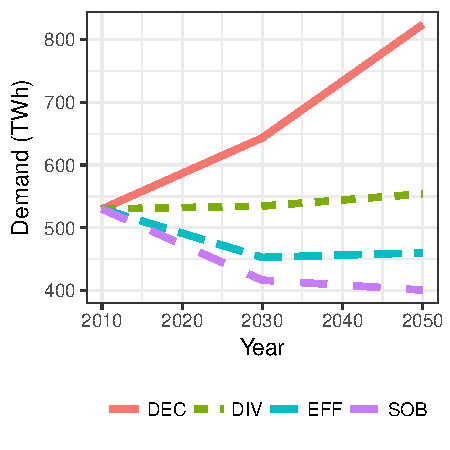
\includegraphics[height=6cm]{figures/dnte_demands.pdf}
	}
	\caption{Characteristics of the four official scenarios in the French national debate \\Source: \citet{DNTE_gt2} and authors' calculations}
	\label{fig:DNTE_scenarios}
\end{figure}

